\section{FSM}
\label{sec:fsm}
Wir betrachten nun etwas genauer, wie wir unser Konzept einer FSM zur 
Kontrollflusssteurung in \textit{C++11} umgesetzt haben. Dazu gehört neben der Wahl 
der Klassenstruktur auch die Einbindung nützlicher Features von C++11, um die
Speicherverwaltung zu optimieren.


%%%%%%
\subsection{Klassenstruktur}
Zur Modellierung einer FSM haben wir uns ein Konzept aus einer Kontroller Klasse \texttt{FSM} und zwei abstrakten Basisklassen \texttt{State} und \texttt{Transition} überlegt. Dabei stellen die abstrakten Basisklassen nur eine standardisiertes Interface bereit und erlauben somit eine schnelle Implementation von neuen, abgeleiteten Klassen.


Erst die abgeleiteten Klassen implementieren eine genaue Funktionalität, wie z.B. einer Wand zu folgen oder eine Transition nach einem bestimmten Ereignis auszulösen. Diese Klassen sind in den dafür vorgesehenen namespaces \texttt{TRAL::STATES} und \texttt{TRAL::TRANSITIONS} zu finden.

\begin{figure}[htbp] 
  \centering
     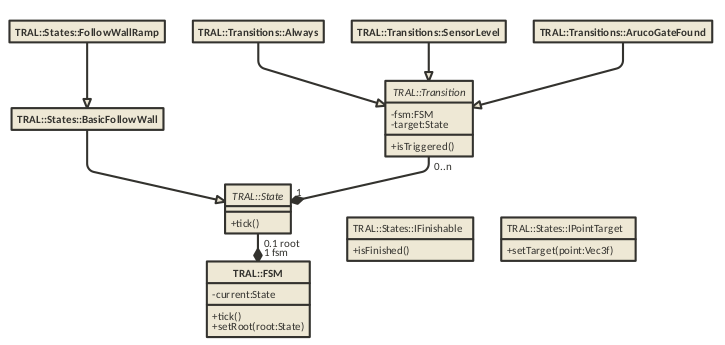
\includegraphics[width=\textwidth]{images/fsm-uml.png}
  \caption{Vereinfachtes Klassendiagram der FSM}
  \label{fig:KlassendiagramFSM}
\end{figure}

%%%%%%
\subsubsection{FSM}
Die Klasse \texttt{FSM} implementiert die komplette Kontrollflusssteuerung und kümmert sich auch um das Laden einer FSM, die zuvor graphisch mit UMLet (siehe Abschnitt 10, graphische Programmierung) erstellt wurde. Ebenso hält diese Klasse immer eine aktuelle Referenz zu dem globalen \texttt{MachineState}. In dieser Klasse sind alle Sensorinformationen aufbereitet konsolidiert.

\paragraph{\texttt{FSM::tick}}

Die wichtigste Funktion dieser Klasse ist die \texttt{tick} Funktion. Diese wird zyklisch vom ROS-Node tral-fsm aufgerufen. Dabei wird der Kontrollfluss an den aktuell aktiven State weitergeben. Wenn nun der aktive State eine neue Ausgabe gesetzt hat und die Kontrolle wieder abgibt, werden nun alle an diesem State befindlichen Transitionen daraufhin überprüft, ob sie ausgelöst haben. Sollte dies der Fall sein, wird eine \texttt{transit} vollzogen.

\paragraph{\texttt{FSM::transit}}

Beim Statewechsel wird zuerst dem aktuell noch aktiven State signalisiert, dass er nun verlassen wird. Dabei kann der State zum Beispiel genutzte Ressourcen wieder freigeben. Darauf folgend wird dem neuen State signalisiert, dass dieser nun betreten wird und nötige Ressourcen belegen kann.


%%%%%%
\subsubsection{State}
Die Klasse \texttt{TRAL::State} ist eine abstrakte Basisklasse, von der alle weiteren States abgeleitet werden. Für unsere Implementierung wurden zum Beispiel folgende States abgeleitet:

\begin{itemize}
	\item ApproachPoint
	\item ArucoGateCenter
	\item BasisFollowWall
	\begin{itemize}
		\item FollowWallRamp
	\end{itemize}
	\item FollowWall
	\item Idle
	\item Motor
	\item Stop
\end{itemize}

Jeder instantiierbarer State muss alle virtuellen Funktionen der State-Klasse implementieren. Dadurch wird gewährleistet, dass die FSM-Klasse mit jeder beliegen State-Implementierung arbeiten kann.

Die statische Funktion \texttt{createFromJson} erlaubt, ein State-Instanz aus einem JSON-Objekt zu erzeugen. Als virtuelles Interface sind die Funktionen \texttt{tick}, \texttt{onEnter}, \texttt{onExit} und weitere Debug-Funktionen vorgesehen.

\texttt{onEnter} und \texttt{onExit} signalisieren das zuvor beschriebene Betreten und Verlassen eines States bei der Ausführung. Die Funktion \texttt{tick} wird für den aktiven State zyklisch ausgeführt und berechnet einen neue Ausgabe. Dabei kann über den globalen \texttt{MachineState} auf die aktuellen Sensorwerte zugegriffen und die Aktoren angesteuert werden.


%%%%%%
\subsubsection{Transition}
Ähnlich der State-Klasse fungiert die \texttt{TRAL::Transition} als abstrakte Basisklasse für alle Transitionen. Ebenso existiert auch eine statische Funktion \texttt{createFromJson}, um gespeicherte Instanzen aus einem JSON-Objekt zu laden. 

Jede Transition gehört zu einem eindeutigen Besitzer \textit{owner} und zu einem eindeutigen Ziel \textit{target}. Sollte der \textit{owner}-State aktuell aktiv sein, wird jede Transition mit der Funktion \texttt{isTriggerd} auf Auslösung durch die FSM Instanz nach der Ausführung des States überprüft.

Für unsere Implementierung haben wir folge Transitionen abgeleitet:

\begin{itemize}
	\item Always
	\item ArucoGateFound
	\item Distance
	\item Finished
	\item SensorLevel
\end{itemize}

%%%%%%
\subsubsection{Interfaces}

Um die Übergabe von Informationen zwischen, zum Beispiel, einem State und einer Transtion zu gewährleisten, haben wir zwei Interfaces für States verwendet. 
States, die das Interface \texttt{IFinishable} einbinden, können entscheiden, wann sie Abgeschlossen sind. Zum Beispiel implementiert der State \texttt{ApproachPoint} dieses Interface und signalisiert die Ankunft an dem definierten Punkt.

Ebenso können States, die das Interface \texttt{ApproachPoint} implementieren, einen Zielpunkt gesetzt bekommen. Dieses Interface wird zum Beispiel auch vom State \texttt{ApproachPoint} implementiert und erlaubt so ein Verlegen des definierten Punktes bei der Ausführung.

So muss der \textit{owner} State der \texttt{Finished} Transition das dazugehörige Interface implementieren. Sollte dies nicht der Fall sein, kommt es zu einem Laufzeitfehler während der Ausführung.
